\chapter{Výsledky experimentů}
V této kapitole jsou shrnuty výsledky, kterých bylo v rámci práce na tématu dizertace dosaženo. Jmenovitě jsou to výsledky navrženého algoritmu Extreme Seeking Entropy (viz kapitola \ref{chap: ESE_vysledky}) a potom použití algoritmu Learning Entropy pro adaptivní fuzzy filtr při detekci změn stavu bioprocesu (viz kapitola \ref{chap:LE_fuzzy}). Výsledky byly publikovány v \cite{ese_mdpi}.
\section{Případové studie detekce novosti algoritmu Extreme Seeking Entropy}\label{chap: ESE_vysledky}
Obsah této kapitoly je shrnutím výsledků publikovaných v MDPI.
\subsection{Případová studie: chaotická časová řada Mackey-Glass a detekce pertubace}
Tento experiment byl proveden pro porovnání s výsledky uvedenými v publikaci \cite{ivoLE1}, která je první publikací o algoritmu LE (viz kapitola \ref{chap:LE}). Experiment spočívá v detekci pertubovaného vzorku v chaotické časové řadě, která je výsledkem řešení Mackey-Glassovy rovnice \cite{mackey}.
\begin{equation}
    \frac{dy(t)}{dt}= \beta \cdot \frac{ y(t-\tau)}{1 + y^\alpha(t-\tau)} - \gamma y(t)
\end{equation}
přičemž parametry $\alpha = 10$, $\beta = 0.2$, $\gamma = 0.1$ and $\tau = 17$ byly vybrány tak, aby řešením této rovnice byla chaotická časová řada. Celkem bylo vygenerováno 701 vzorků. Data v diskrétní časový okamžiku $k=523$ pak byly pertubovány podle následujícího předpisu.
\begin{equation}
    y(523) = y(523) + 0.05 \cdot y(523)
\end{equation}
Výsledná časová řada a detail pertubace je znázorněn na obrázku \ref{fig:mackey_details}. Jako adaptivní filtr byl zvolen QNU (resp. Volterrův filtr) jehož vstupem jsou 4 časově spožděné hodnoty časové řady $y(k-1)$, $y(k-2)$, $y(k-3)$, $y(k-4)$. Hodnoty adaptivních vah tohoto filtru byly adaptovány algoritmem NLMS. Struktura filtru byla zvolena stejně jako v \cite{ivoLE1}. Rychlost učení během experimentu byla nastavena na $\mu=1$. Metoda POT byla zvolena podle rovnice \ref{eq:l1} a délka okna pro detekci novosti algoritmem ESE byla nastavena na $n_s=300$. 
\par 
Výstup adaptivního filtru a chyba predikce jsou znázorněny na obrázku \ref{fig:mackey_results}. Výsledky metod detekce novosti jsou zobrazeny na obrázku \ref{fig:mackey_results_nd}. Z obrázku je patrné, že globální maximum průběhu $ESE$ odpovídá pertubovaným datům. Globální maximum metod $ELBND$ a $LE$ odpovídá vzorku u něhož byla největší chyba predikce. Hodnoty prahů algoritmu LE byly zvoleny $\boldsymbol{\alpha}=\{4,5,6,7,8,9\}$ a délka okna byla nastavena na $m=30$.


\begin{figure}[!ht]
    \centering
    \includegraphics[scale=0.56]{IMG/mdpi/mackeydetails_diz.eps}
    \caption{Horní graf zobrazuje celou datovou řadu. Spodní grafy zobrazují detail pertubovaného vzorku v diskrétní časový okamžik $k=523$.}
    \label{fig:mackey_details}
\end{figure}
\begin{figure}[!ht]
    \centering
    \includegraphics[scale=0.56]{IMG/mdpi/mackey_results.eps}
    \caption{Graf (a) zobrazuje datovou řadu s pertubací (černá plná čára) a výstup adaptivního filtru (tečkovaná zelená čára). Pertubovaný vzorek je označen černou šipkou. Graf (b) zobrazuje velikost chyby predikce $e$ (resp. její absolutní hodnotu). Na grafu (c) jsou znázorněny přírůstky adaptivních vah filtru (resp. absolutní hodnotu těchto přírůstků).}
    \label{fig:mackey_results}
\end{figure}

\begin{figure}[!ht]
    \centering
    \includegraphics[scale=0.56]{IMG/mdpi/mackey_results_nd.eps}
    \caption{Graf (a) zobrazuje hodnotu ESE. Prvních 300 vzorků je hodnota ESE nulová, protože délka okna pro vyhodnocování novosti $n_s=300$. Graf (b) zobrazuje výsledky algoritmu ELBND. Prvních 300 výsledků ELBND je pro názornost vynecháno. Graf (c) zobrazuje výsledky algoritmu LE.}
    \label{fig:mackey_results_nd}
\end{figure}

\subsection{Případová studie: detekce změny rozptylu šumu v náhodném datovém toku}
Tato případová studie je navržená na základě problému, který se vyskytuje v použití hybridních navigačních systémů využívajících GPS (Global Positioning System) senzory pro navigaci výpočtem \cite{dead}. Smyslem experimentu je demonstrovat možnost využití algoritmu ESE pro detekci změn rozptylu šumu v náhodných datech.
\par
Uvažujme dva vstupy $x_1(k)$ a $x_2(k)$ a výstup generátoru signálu $y(k)$ takový, že
\begin{equation}
y(k)=x_1(k)+x_2(k)+x_1(k)\cdot x_2(k)+v(k)
\end{equation}
kde člen $v(k)$ reprezentuje aditivní Gaussovský šum který je přidán k výstupu generátoru $y(k)$. Přidaný šum má nulovou střední hodnotu a směrodatnou odchylku $\sigma_n=0.1$, takže $v(k)\sim N(0,1)$. Hodnoty vstupů jsou v každém diskrétním časovém okamžiku vybrány náhodně z rovnoměrného rozdělení na intervalu $\langle 0,\rangle$. V diskrétním časovém okamžiku $k=500$ dojde ke změně směrodatné odchylky šumu na hodnota $\sigma_n=0.2$, $v(k) \sim N(0,0.2)$.
\par 
Adaptivní filtr v tomto experimentu byl QNU ve tvaru
\begin{equation}
\hat{y}(k)=w_1\cdot x_1(k) + w_2\cdot x_2(k)+w_3\cdot x_1(k)\cdot x_2(k)
\end{equation}
tak,  že jeho struktura odpovídá struktuře generátoru signálu. Adaptivní parametry filtru byly adaptovány algoritmem GNGD. Rychlost učení byla nastavená jako $\mu=1$. Metoda POT byla zvolena podle \ref{eq:l2} a délka okna $n_s=500$. Výsledky experimentu jsou zobrazeny na obrázku \ref{fig:noise_changed}. Apriorní hodnoty parametrů GPD byly stanoveny na základě 500 vzorků, které nejsou v následujícím obrázku \ref{fig:noise_changed} zobrazeny. Globální maximum ESE odpovídá změně směrodatné odchylky šumu $\sigma_n$. Detekce pomocí algoritmů LE a ELBND je o několik vzorků opožděná. Pro výpočet LE byl použit vztah \ref{eq:le_direct_padasip} a délka okna byla nastavena na $M=300$.

\begin{figure}[ht!] 
    \centering
    \includegraphics[scale=0.60]{IMG/mdpi/noise_change.eps}
    \caption{Na grafu (a) jsou zobrazeny data z generátoru (modrá) a výstup z adaptivního filtru (zelená). Na grafu (b) je vynesena chyba filtru $e(k)$. Graf (c) zobrazuje velikosti přírůstků adaptivních parametrů filtru. Na grafu (d) jsou zobrazeny hodnoty ESE. V diskrétní časový okamžik $k=500$ je patrný značný nárůst v ESE, který reflektuje změnu směrodatné odchylky aditivního šumu. Na dalších grafech (e) a (f) jsou zobrazeny výsledné hodnoty algoritmů ELBND a LE.}
    \label{fig:noise_changed}
\end{figure}

\subsection{Případová studie: detekce skokové změny parametrů generátoru signálu}
\#TODO
\subsection{Případová studie: detekce náhlé absence šumu}
In this experiment it is shown, that the slightly reformulated algorithm can detect also deal with immediate decrease of learning effort. Assume, that instead of unusually high learning effort, we want to focus on unusually low learning effort. The only change in the proposed algorithm is, that we will use POT method to get $l$ the smallest weight updates and based on those updates the parameters of GPDs are estimated.
The scheme of this experiment is similar to previous. Assuming two inputs $x_1(k)$ and $x_2(k)$ and output $y(k)$ that are related by the equation (\ref{eq:x1x2}). But in this case, at discrete time index $k=500$, the noise is removed, so the equation (\ref{eq:x1x2}) for $k \geq 500$ takes the form
\begin{equation}
    y(k)=x_1(k)+x_2(k)+x_1(k)x_2(k).
\end{equation}
The QNU was chosen for obtained data processing. The number of inputs to QNU was set to $n=2$ so the inputs are
\begin{equation}
    \textbf{x} = [x_1(k-1), x_2(k-1)]
\end{equation}
so the adaptive filter has totally 3 adaptive weights. \textcolor{red}{The structure of the adaptive filter was chosen to correspond with the structure of the signal generator.} The parameters are updated with every new obtained sample with the GNGD algorithm. The learning rate during the experiment was constantly set to $\mu = 1$. The POT method was chosen according to (\ref{eq:l1}) with $n_s=500$. The following \autoref{fig:noise_ext} shows, that the peak in $ESE$ corresponds with the noise disappearance. \textcolor{red}{The $LE$ and $ELBND$ methods failed to detect the noise dissapearance. For $ELBND$ this results can be expected as the values of the $ELBND$ are high for high prediction error and high adaptive weight increments.}
\begin{figure}[h!] 
    \centering
    \includegraphics[scale=0.65]{IMG/mdpi/noise_ext.eps} 
    \caption{Noise disappearance detection. The graph (a) shows the data series (blue) and the  output of the predictor (green). The graph (b) shows the value of predictors error. The graph (c) shows the absolute value of adaptable parameters increments. The graph (d) shows the $ESE$ novelty score. For discrete time index $k \geq 500$ the noise is removed from the signal which corresponds with peak in $ESE$. \textcolor{red}{Graph (e) and (f) contains results of ELBND and LE methods.}}
    \label{fig:noise_ext}
\end{figure}
\subsection{Případová studie: detekce změny trendu}
\#TODO
\subsection{Případová studie: detekce epilepsie v myším EEG}
\#TODO
\subsection{Vyhodnocení úspěšnosti detekce skokové změny parametrů generátoru signálu}
\#TODO
\section{Vyhodnocení úspěšnosti detekce změny trendu a evaluace ROC křivky}
\#TODO
\section{Vyhodnocení výpočetní náročnosti metod odhadu parametrů zobecněného Paretova rozdělení}
Výsledky v této podkapitole byli publikovány v (můj shit). Cílem bylo určit výpočetní čas výpočtu parametrů GPD v typické aplikaci pro použití algoritmu ESE, který byl, v tomto případě, testován ne experimentu detekce skokové změny parametrů generátoru signálu.
\subsection{Motivace}
Detekce novosti v reálném čase je úloha, která nalézá své uplatnění nejen v oblasti detekci a diagnostiky v průmyslových aplikacích \cite{fault}, ale také např. v detekci narušení počítačových sítí \cite{data_streams} nebo v zabezpečovacích systémech \cite{surveilance}. Další oblastí uplatnění je např. mobilní robotika, která je specifická tím, že robot má k dispozici pouze limitovaný výpočetní výkon \cite{robotics_marslan,robotics}. Pro metody detekce novosti v reálném čase je tedy důležité, aby vynikali dostatečně nízkou výpočetní náročností. Z tohoto důvodu byli otestovány tři různé metody výpočtu parametrů GPD (viz kapitola \ref{chap:gpd}, protože tento výpočet je z hlediska použití algoritmu ESE potenciálně limitující z hlediska využitelnosti v aplikacích detekce v reálném čase. Jmenovitě byli otestovány tyto metody: metoda maximální věrohodnosti (ML), metoda momentů (MOM) a metoda kvazi-maximální věrohodnosti (QML) (více viz kapitola \ref{chap:gpd}). Výpočetní čas potřebný k určení parametrů GPD pomocí těchto metod byl vyhodnocen při experimentu, ve kterém dojde ke skokové změně parametrů generátoru signálu.
\subsection{Specifikace experimentu}
Vzhledem k povaze experimentu, který slouží k vyhodnocení výpočetní náročnosti různých metod určení parametrů GPD, a nikoliv k detekci novosti v nějakém komplexním procesu, byl zvolen jednoduchý lineární kombinační filtr (LNU), jehož výstup v diskrétním časovém okamžiku $k$ je definován jako
\begin{equation}\label{eq:gene_ese_1}
\hat{y}(k)=w_1\cdot x_1(k)+w_2\cdot x_2(k)+w_3\cdot x_3(k)
\end{equation}
a tento filtr je adaptován algoritmem NLMS (viz kapitola \ref{chap:nlms}), přičemž rychlost učení $\mu$ byla nastavena jako $\mu=0.8$.
\par 
Pro výstup generátoru signálu platí vztah
\begin{equation}
y(k)=x_1(k)+x_2(k)+x_3(k)+v(k)
\end{equation}
pro všechny $1 \leq k \leq 200$. Člen $v(k)$ reprezentuje aditivní gaussovský šum s nulovou střední hodnotou a směrodatnou odchylkou $\sigma_{noise}=0.1$. V diskrétním časovém okamžiku $k=201$ dojde ke změně generátoru signálu a jeho výstup přejde do tvaru
\begin{equation}
y(k)=0.7\cdot x_1(k)+1.2\cdot x_1(k)+1.1 \cdot x_1(k) + v(k)
\end{equation}
pro $201 \leq k \leq 400$. Hodnota všech vstupů generátoru signálu je v každém časovém okamžiku $k$ vybrána ze standartního rozdělení normálního rozdělení, takže $i$-tý vstup $x_i\sim \mathcal{N}(0,1)$. Změna parametrů signálu byla vybrána tak, aby nedošlo ke změně střední hodnoty signálu $y(k)$.
\par
Délka okna pro odhad parametrů GPD bylě během experimentu nastavena na $n_s=1200$. Metoda POT byla zvolena podle REF na 10\%. Před experimentem bylo pořízení 1200 vzorků vygenerovaných generátorem signálu definovaným vztahem \ref{eq:gene_ese_1}, na něž byla použita metoda POT, tak aby při experimentu v diskrétní časový okamžik $k=1$ byla hodnota ESE relevantní.
\par
Experiment byl proveden na PC s procesorem Intel(R) Core(TM) i5-7400 se 4mi jádry s taktovací frekvencí 3001 MHz a operační pamětí o velikosti 32 GB. Operační systém byl Windows 10 Pro, 64-bitová verze 10.0.18362. Kód byl napsán v Python 3.6.1 a byly použity knihovny Numpy 1.17.0 a Scipy 1.4.1.
Pro

\begin{figure}[h!]
	\label{fig:par_output}
	\centering
	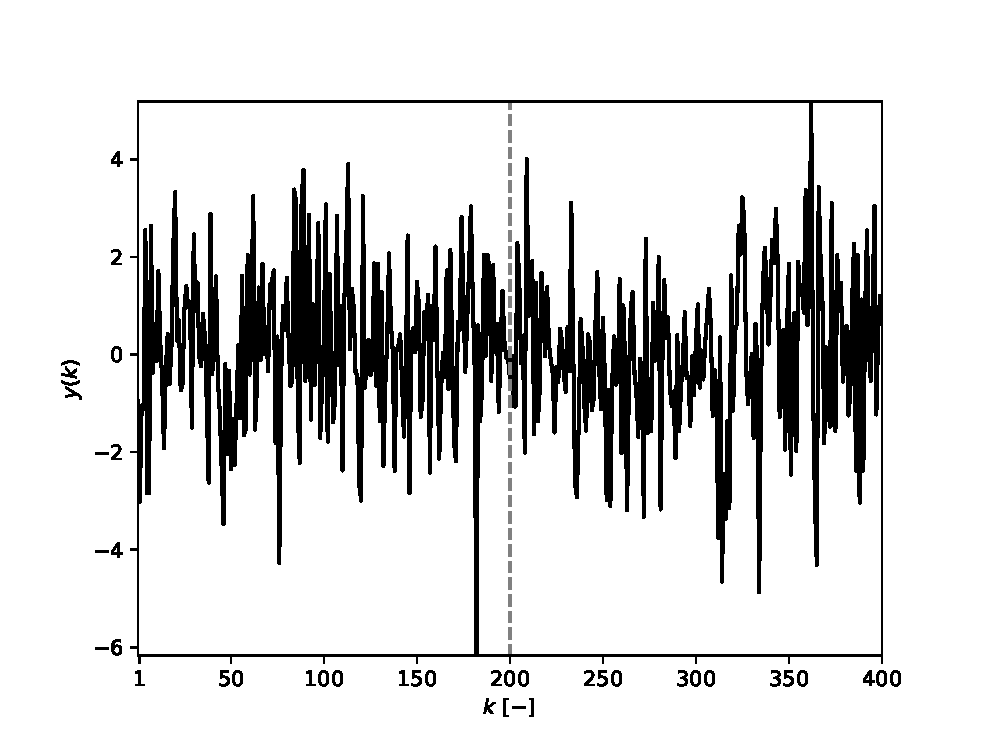
\includegraphics[scale=0.71]{IMG/appel_par/par_output.eps}
	\caption{Výstup adaptivního filtru během experimentu. Skoková změna parametrů generátoru signálu je zvýrazněná svislou vodorovnou čarou v diskrétním časovém okamžiku $k=200$.}
\end{figure}

\subsection{Výsledky a diskuze}


\begin{figure}[h!]
	\label{fig:par_ese}
	\centering
	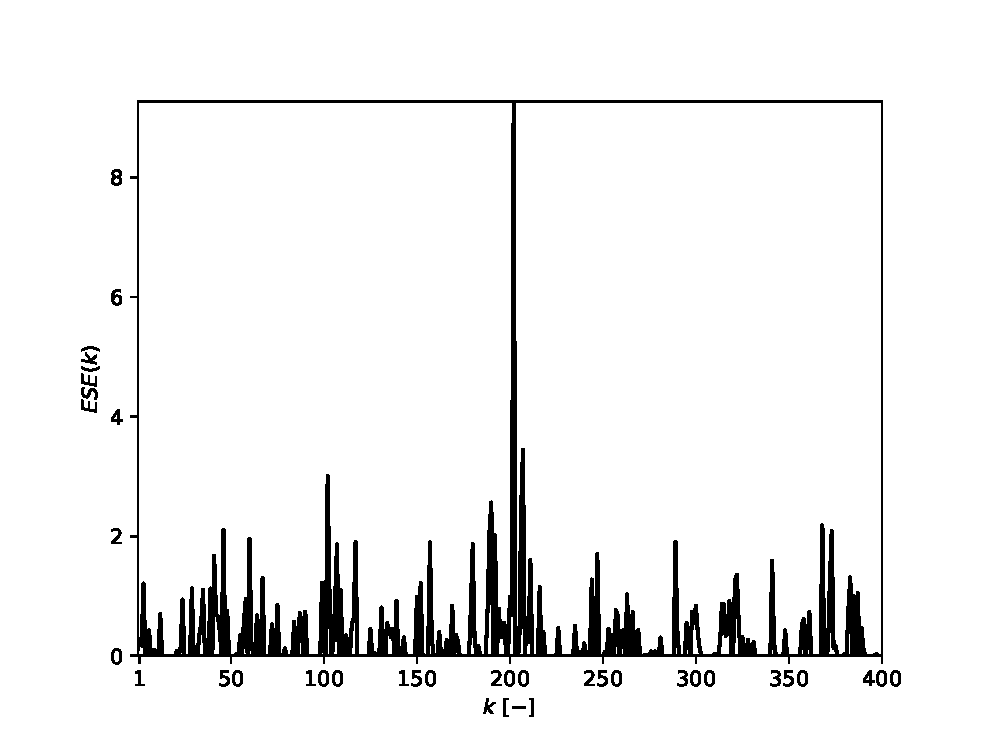
\includegraphics[scale=0.71]{IMG/appel_par/par_ese.eps}
	\caption{Hodnota ESE během experimentu. Globální maximum odpovídá změně parametrů generátoru signálu, resp. úspěšné detekci novosti.}
\end{figure}

\begin{figure}[h!]
	\label{fig:par_mu}
	\centering
	\includegraphics[scale=0.71]{IMG/appel_par/par_mu.eps}
	\caption{Hodnota parametru $\mu$ GPD pro všechny tři adaptivní váhy $w_1$, $w_2$, $w_3$ během experimentu detekce změn parametrů generátoru signálu. Svislá čára v diskrétním časovém okamžiku $k=200$ znázorňuje skokovou změnu parametrů generátoru signálu.}
\end{figure}

\begin{figure}[h!]
	\label{fig:par_gamma}
	\centering
	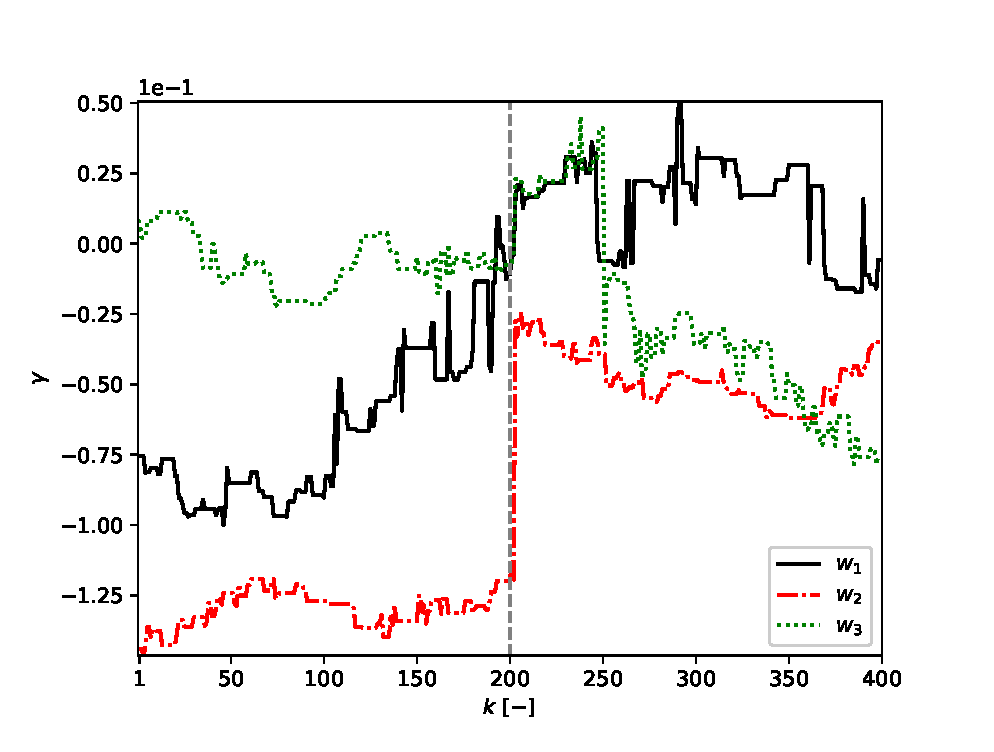
\includegraphics[scale=0.71]{IMG/appel_par/par_gamma.eps}
	\caption{Hodnota parametru $\gamma$ GPD pro všechny tři adaptivní váhy $w_1$, $w_2$, $w_3$ během experimentu detekce změn parametrů generátoru signálu. Svislá čára v diskrétním časovém okamžiku $k=200$ znázorňuje skokovou změnu parametrů generátoru signálu.}
\end{figure}

\begin{figure}[h!]
	\label{fig:par_sigma}
	\centering
	\includegraphics[scale=0.71]{IMG/appel_par/par_mu.eps}
	\caption{Hodnota parametru $\sigma$ GPD pro všechny tři adaptivní váhy $w_1$, $w_2$, $w_3$ během experimentu detekce změn parametrů generátoru signálu. Svislá čára v diskrétním časovém okamžiku $k=200$ znázorňuje skokovou změnu parametrů generátoru signálu.}
\end{figure}
Průměrný čas výpočtu $\overline{t}$ parametrů všech tří GPD (počet GPD odpovídá počtu adaptivních parametrů filtru) a odpovídající směrodatné odchylky $\sigma_t$ jsou uvedeny v následující tabulce \ref{tab:par_results}. Čas výpočtu je určený pro jeden experiment (400 vzorků).
\begin{table}[h!]

\centering
\caption{Tabulka průměrných časů výpočtu pro jednotlivé adaptivní váhy a odpovídajících směrodatných odchylek vybraných metod výpočtu parametrů GPD}
\begin{tabular}{|l|l||l|l|}
\hline
 & Metoda & $\overline{t}$ {[}ms{]} & $\sigma_t$ {[}ms{]} \\ \hline \hline
\multirow{3}{*}{$w_1$} & ML & $26.198$ & $3.396$ \\ \cline{2-4} 
 & QML & $0.354$ & $0.478$ \\ \cline{2-4} 
 & MOM & $\textbf{0.076}$ & $0.264$ \\ \hline
\multirow{3}{*}{$w_2$} & ML & $26.718$ & $2.302$ \\ \cline{2-4} 
 & QML & $0.337$ & $0.471$ \\ \cline{2-4} 
 & MOM & $\textbf{0.064}$ & $0.244$ \\ \hline
\multirow{3}{*}{$w_3$} & ML & $24.982$ & $1.964$ \\ \cline{2-4} 
 & QML & $0.395$ & $0.489$ \\ \cline{2-4} 
 & MOM & $\textbf{0.060}$ & $0.238$ \\ \hline

\end{tabular}
 \label{tab:par_results}
\end{table}

Z uvedených výsledků je patrné, že nejrychlejší metoda je MOM. Podstatnou nevýhodou této metody pro využití v aplikacích, které vyhodnocují data v reálném čase je její omezení na hodnoty parametrů GPD (viz kapitola \ref{chap:gpd}). Pokud parametry uvedené omezení nesplňují, vypočtené hodnoty nepřesné (resp. nesmyslné) a tedy nepoužitelné pro algoritmus ESE, který začne produkovat nepřesné výsledky. Z pohledu úlohy detekce novosti je diskutabilní, zda-li můžeme garantovat, že sledovaný proces po celou dobu bude splňovat uvedené omezení.
\par
Metoda, jejíž výpočetní čas byl nejvyšší je ML, což je vzhledem k iterativnímu určení parametrů GPD očekávatelné. Nevýhoda použití této metody tkví v  nemožnosti určit minimální resp. maximální počet iterací. Jednou z možností jak zrychlit nalezení parametrů je využití apriorní informace o hodnotách těchto parametrů. V rámci experimentu však byla využita pouze apriorní informace o parametru $\mu$, který odpovídá nejmenší hodnotě přírůstku vah, které byli získány metodou POT aplikovanou na plovoucí okno délky $n_s$.
\par
Dobrým kompromisem mezi výše uvedenými metodami je použití metody QML. Výpočetní čas této metody byl v uvedeném experimentu o dva řády kratší než ML a asi pětkrát delší než MOM. Pro každou z vyhodnocovaných vah byl kratší než $500$ $\mu s$.
\par 
Z provedeného experimentu je patrné, že použití algoritmu ESE pro aplikace v reálném čase je limitováno počtem parametrů filtru a rychlostí vzorkování monitorovaného procesu. 





\section{Případová studie použití algoritmu Learning Entropy a adaptivního fuzzy filtru pro detekci změn stavů bioprocesu} \label{chap:LE_fuzzy}
Cílem této studie je ověřit, že algoritmus LE, který byl doposud publikován s adaptivními filtry typu LNU a HONU, je možné použít i pro jiné typy adaptivních filtrů. Pro provedenou studii tak byl vybrán adaptivní fuzzy filtr (viz kapitola \ref{chap:fuzzyf}).
\subsection{Popis bioprocesu a specifikace problému}
Podle \cite{fermentace} je pro fermentační procesy, které probíhají v dávkovém režimu je podstatné, aby probíhalo správně dávkované živení substrátem. Pro tyto procesy je specifické, že se při nadměrných koncentracích stává substrát pro mikroorganismy toxickým a může dojít k tzv. přeživení a tím i zahubení těchto mikroorganismů. Naopak, v důsledku nedostatečného zábovení živinami může dojít k odumření kultivovaného organismu. Z tohoto pohledu se je tedy důležité v závislosti na koncentraci substrátu a stavu populace mikroorganismů měnit i strategii pro řízení procesu kultivace. Historicky byl stav bioprocesu klasifikován expertem, přičemž vyhodnocení bylo poměrně časově náročné a nebylo neobvyklé, že různí experti docházeli k rozdílným závěrům. Protože výnos fermentačního procesu je zásadním způsobem ovlivněn správnou klasifikací stavu ve kterém se právě nacházi, bylo by vhodné klasifikaci automatizovat a pokud možno zvýšit její přesnost. Tomuto problému je právě věnována publikace \cite{fermentace}, která řeší problém automatické klasifikace stavů bioprocesu kultivace bakterie \textit{Pseudomonas putida KT2442}. V této publikaci je navržen komplexní algoritmus pro online klasifikaci stavů bioprocesu. Autoři zde rozlišují celkem tři stavy bioprocesu kultivace \textit{Pseudomonas putida KT2442}, konkrétně:
\begin{enumerate}
    \item normální živení
    \item přeživení
    \item nedoživení
\end{enumerate}
Navržený algoritmus vyhodnocuje přísun vstupujících živin (Fm), respektive substrátu, a změny a trendu rozpuštěného kyslíku (DO), který je produkován bakteriemi \textit{Pseudomonas putida} a pomocí hřebenové regrese (v literatuře se vyskytuje také pod názvem Tichonova regularizace) je určován vývoj populace bakterií respektive stav bioprocesu. Vzhledem k tomu, že modely vývoje populace pro jednotlivé stavy jsou různé, mohlo by v průběhu experimentu dojít i k podstatným změnám v adaptivním modelu v okamžicích změn stavů kultivace. Tyto změny se mohli projevit neobvykle velkými přírůstky adaptivních parametrů. 
\par
Protože algoritmus Learning Entropy využívá přírůstku adaptivních parametrů, mohl by být vhodným nástrojem pro detekci změn stavů bioprocesu. Předpokládáme, že tedy existuje souvislost mezi změnami stavu bioprocesu a nárůstem Learning Entropy. Přestože může být proces kultivace bakterií \textit{Pseudonomas Putidas} modelován různými a různě složitými modely, pro využití algoritmu Learning Entropy se jeví výhodné použít jednoduché prediktory nebo sledovače. Dosud publikované články využívali pro algoritmus LE pouze FIR filtry, případně Volterrovy filtry, které mají adaptivní parametry v lineární závislosti. V tomto experimentu je použit adaptivní fuzzy filtr, jehož struktura je specifikována v kapitole \ref{chap:fuzzyf} a k jehož adaptaci byl použit algoritmus, který je uveden v kapitole \ref{chap:gd}.
\par
Použitý adaptivní fuzzy filtr má 9 pravidel ($M=9$), jehož $l$-té pravidlo je ve tvaru
\begin{equation}
    IF\;do(k-1)\; is\; A_1^l\;AND\;do(k-6)\;is\;A_2^l\;AND\;do(k-19)\;is\;A_3^l\;THEN\;do(k)\;is\;B^l
\end{equation}
kde $A_i^l$ je množina ve vstupním prostoru $U \subset R^3$ a $B^l$ je fuzzy množina ve výstupním prostoru $V \subset R$. V uvedeném pravidle jsou $do(k-1)$, $do(k-6)$, $do(k-19)$ a $do(k)$ lingvistické proměnné, které vyjadřují koncentraci rozpuštěného kyslíku $do$ v v diskrétních časových okamžicích $k$, $k-1$, $k-6$ respektive $k-19$, kde $k$ je diskrétní časový index. Vzhledem k tomu, že uvedený adaptivní fuzzy filtr používá Gaussovské funkce příslušnosti (viz kapitola \ref{chap:fuzzyf} je zobrazení popisující jeho výstup ve tvaru
\begin{equation}
    \hat{y}(\textbf{x}(k))=\frac{\sum_{j=1}^9 \overline{b}^j\Big[\prod_{i=1}^3 exp\Big(-\Big(\frac{x_i-\overline{x}_i^j}{\sigma_i^j}\Big)\Big)\Big]}{\sum_{j=1}^9 \Big[\prod_{i=1}^3 exp\Big(-\Big(\frac{x_i-\overline{x}_i^j}{\sigma_i^j}\Big)\Big)\Big]}
\end{equation}
kde vektor $\textbf{x}(k)$ je
\begin{equation}
    \textbf{x}(k)=[do(k-1),do(k-6),do(k-19)].
\end{equation}\
Protože hodnota koncetnrace rozpuštěného kyslíku je uváděna v procentech, platí pro všechna $x_i\in \langle 0;100\rangle$. K adaptování výše uvedeného filtru byl použit algoritmus gradient descent (viz kapitola \ref{chap:gd}. Maximální počet epoch byl stanoven na $q_{max}=100$ a požadovaná chyba predikce mezi výstupem adaptivního filtru a naměřenými daty na $\epsilon=0,001$. Rychlost učení byla během experimentů nastavena na $\mu=1$.
\par
Pro vyhodnocení novosti byla použita přímá verze algoritmu LE, takže
\begin{equation}\label{eq:le_putida}
    E(k)=max\{0, \sum_{j=1}^9 z(\abs{\Delta \overline{b^j})}-\beta\}
\end{equation}
kde funkce $z$ je dána rovnicí (XY) a $\beta$ je citlivostní parametr. Pro vyhodnocení novosti jsou tedy použity změny polohy středů množin ve výstupním prostoru, nikoliv změny parametrů fuzzy množin ve vstupním prostoru.

\subsection{Experiment a zhodnocení}
Experiment s použitím algoritmu LE a adaptivního fuzzy filtru byl uskutečněn na datech z kultivace bakterie \textit{Pseudonomas Putida}, který byl uskutečněn na Ústavu počítačové a řídicí techniky VŠCHT Praha. Celkem byly zpracovávány hodnoty ze dvou kultivací. Přestože bylo během experimentu měřena sada různých veličin (např. teplota, pH, atd.), osvědčil se pro použití LE signál rozpustěného kyslíku $do$ $[\%]$. Během experimentu bylo použito vzorkování $T=1$ $min$, což je vzhledem k rychlosti celého procesu dostatečně rychlé vzorkování. Počáteční nastavení parametrů adaptivního fuzzy filtru bylo provedeno tak, jak je popsáné v kapitole \ref{chap:gd}. Podstatný vliv na výsledek detekce změn stavu bioprocesu měla volba volba délky okna pro vyhodnocení změn adaptabilních parametrů filtru $M_{ND}$. Na základě experimentů s různými délkami byla nakonec zvolena délka okna $M_{ND}=20$.
\par
Na následujících obrázcích je znázorněn průběh signálu $do$ během první kultivace (viz obrázek \ref{fig:artep_1}), chyba predikce (viz obrázek \ref{fig:artep_3}) a odpovídající hodnoty $LE$ společně se stavy bioprocesu (viz obrázek \ref{fig:artep_4}). Význam stavů bioprocesu znázorněných na obrázku \ref{fig:artep_3} respektive obrázku \ref{fig:artep_6} jsou: 1 - nedoživení, 2 - živení, 3 - přeživení. Aby byli detekovány všechny změny stavu bioprocesů, byla stanovena hodnota parametru $\beta=2,58$ (viz rovnice \ref{eq:le_putida}).
\par
Data z druhé kultivace byla použita k ověření správného nastavení parametru $\beta$.  Obrázek \ref{fig:artep_2} zobrazuje průběh signálu $do$ během druhého experimentu. Chyba predikce adaptivního fuzzy filtru je zobrazena na obrázku \ref{fig:artep_5}.  Obrázek \ref{fig:artep_6} zobrazuje stavy bioprocesu během kultivace a odpovídající hodnoty $LE$. S tímto nastavením parametru $\beta$ se podařilo detekovat pouze tři změny bioprocesu. Nicméně pro jiné hodnoty délky okna $M_{ND}$ a hodnoty parametru $\beta$ se tyto změny detekovat podařilo. Je tedy zřejmé, že pro praktické použití je správná volba obou parametrů zásadní. Vzhledem k malému množství dat a časové náročnosti kultivace nebylo možné použít nějakou validační metodu. 

\begin{figure}
    \centering
    \includegraphics[scale=0.8]{IMG/artep/artep17_1.png}
    \caption{Průběh signálu $do$ během první kultivace}
    \label{fig:artep_1}
\end{figure}

\begin{figure}
    \centering
    \includegraphics[scale=0.8]{IMG/artep/artep17_3.png}
    \caption{Chyba predikce $e$ během první kultivace}
    \label{fig:artep_3}
\end{figure}

\begin{figure}
    \centering
    \includegraphics[scale=0.8]{IMG/artep/artep17_4.png}
    \caption{Stav bioprocesu a hodnota $LE$ první kultivace}
    \label{fig:artep_5}
\end{figure}

\begin{figure}
    \centering
    \includegraphics[scale=0.8]{IMG/artep/artep17_2.png}
    \caption{Průběh signálu $do$ během druhé kultivace}
    \label{fig:artep_2}
\end{figure}

\begin{figure}
    \centering
    \includegraphics[scale=0.8]{IMG/artep/artep17_5.png}
    \caption{Chyba predikce $e$ během druhé kultivace}
    \label{fig:artep_4}
\end{figure}

\begin{figure}
    \centering
    \includegraphics[scale=0.8]{IMG/artep/artep17_6.png}
    \caption{Stav bioprocesu a hodnota $LE$ během druhé kultivace}
    \label{fig:artep_6}
\end{figure}




 